\documentclass[draft]{agujournal2019}
\usepackage{url} %this package should fix any errors with URLs in refs.
\usepackage{lineno}
%\usepackage[inline]{trackchanges} %for better track changes. finalnew option will compile document with changes incorporated.
\usepackage{soul}
\usepackage{gensymb}
\usepackage{placeins}
\usepackage{multirow}
\usepackage{setspace}
\usepackage{float}

\linenumbers
\onehalfspacing

\draftfalse

\journalname{Water Resources Research}


\begin{document}


\title{Automated Input Variable Selection for Analog Methods Using Genetic Algorithms}

\authors{P. Horton\affil{1}, O. Martius\affil{1}, and S. L. Grimm\affil{2}}

\affiliation{1}{Institute of Geography, Oeschger Centre for Climate Change Research, University of Bern, Bern, Switzerland}
\affiliation{2}{Physikalisches Institut, University of Bern, Gesellschaftsstrasse 6, 3012 Bern, Switzerland}

\correspondingauthor{Pascal Horton}{pascal.horton@giub.unibe.ch}


\begin{keypoints}
\item Genetic algorithms were successful in selecting relevant input variables for the prediction of precipitation by analog methods
\item The analogy criteria were automatically selected, resulting in the discovery of a new promising criterion
\item The optimization resulted in a structure combining different predictors into a single level of analogy, while outperforming stepwise methods
\end{keypoints}


\begin{abstract}

Analog methods (AMs) have long been used for precipitation prediction and climate studies. However, they rely on manual selections of parameters, such as the predictor variables and analogy criterion. Previous work showed the potential of genetic algorithms (GAs) to optimize most parameters of AMs. This research goes one step further and investigates the potential of GAs for automating the selection of the input variables and the analogy criteria (distance metric between two data fields) in AMs. Our study focuses on daily precipitation prediction in central Europe, specifically Switzerland, as a representative case.  
Comparative analysis against established reference methods demonstrates the superiority of the GA-optimized AM in terms of predictive accuracy. The selected input variables exhibit strong associations with key meteorological processes that influence precipitation generation. Further, we identify a new analogy criterion inspired by the Teweles-Wobus criterion, but applied directly to grid values, which consistently performs better than other Euclidean distances. It shows potential for further exploration regarding its unique characteristics. In contrast to conventional stepwise selection approaches, the GA-optimized AM displays a preference for a flatter structure, characterized by a single level of analogy and an increased number of variables.
Although the GA optimization process is computationally intensive, we highlight the use of GPU-based computations to significantly reduce computation time. Overall, our study demonstrates the successful application of GAs in automating input variable selection for AMs, with potential implications for application in diverse locations and data exploration for predicting alternative predictands.


\end{abstract}


\section{Introduction}

Analog methods (AMs) are statistical downscaling techniques \cite{Maraun2010} that rely on inherent relationships between meteorological predictors, usually at a synoptic scale, and local weather \cite{Lorenz1956, Lorenz1969}. AMs look for similar meteorological situations in the past to that of a target date of interest. They provide a conditional prediction based on the observed predictand values at these analog dates. Daily precipitation has been the predictand of interest, either in the context of operational forecasting \cite<e.g.>[]{Hamill2006, Bliefernicht2010, Marty2012, Horton2012, Hamill2015, BenDaoud2016}, climate change studies \cite<e.g.>[]{Dayon2015, Raynaud2016b}, or past climate reconstruction \cite{Caillouet2016}. AMs are also used for other predictands, such as precipitation radar images \cite{Panziera2011, Foresti2015a}, temperature \cite{DelleMonache2013, Caillouet2016, Raynaud2016b, Jezequel2017}, wind \cite{DelleMonache2013, DelleMonache2011, Vanvyve2015, Alessandrini2015, Junk2015, Junk2015c}, and solar radiation or power production \cite{Alessandrini2015a, Bessa2015, Raynaud2016b}.

AMs may consist of a stepwise selection of similar meteorological situations based on multiple predictors organized in different consecutive levels of analogy, each of which conditions the subsequent selection. Each predictor consists of a specific meteorological variable at a specific time and vertical level (if relevant). The similarity between two situations is computed using an analogy criterion (distance metric) over a relevant spatial domain. For each level of analogy, a certain number of analogs are selected \cite{Obled2002, Bontron2004}.

AMs for predicting precipitation commonly have a first level of analogy based on the atmospheric circulation. The variable of interest is the geopotential height (Z) at various pressure levels and specific times throughout the day \cite<Table \ref{table:methods};>{Obled2002, Horton2018a}. \citeA{Bontron2004} introduced a second level of analogy based on a moisture index that is the product of the relative humidity at 850~hPa and the total precipitable water (method RM3 in Table \ref{table:methods}). Other consecutive studies selected different pressure levels (method RM4 in Table \ref{table:methods}) or added a wind component to the moisture index \cite{Marty2010, Horton2018a}. \citeA{BenDaoud2016} inserted an additional level of analogy between the circulation and the moisture analogy based on the vertical velocity at 850~hPa (methods RM6 in Table \ref{table:methods}) and named it "SANDHY" for Stepwise Analog Downscaling method for Hydrology \cite{BenDaoud2016, Caillouet2016}.

To calibrate the method, a semi-automatic sequential procedure \cite{Bontron2004, Radanovics2013, BenDaoud2016} has often been used to optimize the size of the domain and the number of analogs. However, the predictor variables, vertical levels, temporal windows (time of the day), and analogy criteria were selected manually. This manual selection requires the comparison of numerous combinations and a comprehensive assessment of some parameter ranges. Moreover, the sequential calibration procedure successively calibrates the different levels of analogy, and thus it does not handle parameters inter-dependencies. Considering these limitations, \citeA{Horton2017a} introduced a global optimization of the AM using genetic algorithms (GAs). Using this approach, an automatic and objective selection of the temporal windows, the vertical levels, the domains, and the number of analogs became possible, improving the method's prediction skills \cite{Horton2018a}. A weighting of the predictor variables has also been introduced. The only parameters left for a manual selection were the meteorological variables and the analogy criteria.

Selecting predictors for precipitation prediction with AMs in Europe has been the focus of multiple studies aiming to improve prediction skills \cite{Obled2002, Bontron2004, Gibergans-Baguena2007, Radanovics2013, BenDaoud2016}. Thus, the relevant predictors are likely to be known nowadays and supported by expert knowledge. However, transferring AMs to a region with different climatic conditions or to another predictand would involve reconsidering the selected meteorological variables. This work aims to test a fully automatic optimization of all AM parameters, including the selection of the meteorological variables and even the analogy criteria, using GAs. GAs have already been used for input variable selection (IVS) in other contexts \cite{Dheygere2003, Huang2007, Cateni2010, Gobeyn2017}.

We here seek to assess the potential of GAs for input variable selection in the context of the analog method. Moreover, we want to test the GAs' ability to jointly select the distance metric in addition, i.e., the analogy criteria. To compare with well-established AMs, daily precipitation in central Europe, specifically in Switzerland, has been chosen as predictand. Also, as is often the case, the AMs were optimized in the perfect prognosis framework, using predictors from reanalyses. This work focuses mainly on the proof of concept of automatic input variable selection for AMs rather than the details of the obtained results for the case study.

The paper is organized as follows. Section \ref{material_methods} describes the datasets, the fundamentals of AMs, the characteristics of the GAs implementation, the software used, and the experiment setup details. Section \ref{results} presents the results of different analyses, such as the selection of the best predictor variable, the relevance of various AM structures, and the skill of the optimized methods. Section \ref{discussion} discusses some findings of the work. Finally, section \ref{conclusions} summarizes the main contributions of the work and open perspectives for applications of the developed approach.


\section{Material and Methods}
\label{material_methods}

\subsection{Data}
\label{data}

The target variable (predictand) is daily precipitation derived from the RhiresD gridded dataset from MeteoSwiss. It is a daily aggregation (from 06~UTC of day D to 06~UTC of day D+1) at a 2~km resolution with data from 1961 onward. It is produced using an interpolation scheme between gauging stations \cite{Frei1998}. The gridded data was here spatially aggregated across 25 catchments of about 200~km$^2$ (Table \ref{catchments}). These catchments were chosen to cover the different climatic regions of Switzerland \cite{Schuepp1980}, as illustrated in Fig.~\ref{map}.


\begin{figure}[hbt]
	\noindent\includegraphics[width=140mm]{figures/map.jpg}
	\caption{Location of the 25 selected catchments in Switzerland along with the climatic regions (dashed lines) and the river network (source: SwissTopo, HADES).}
	\label{map}
\end{figure}


\begin{table}[hbt]
	\centering
	\caption{Characteristics of the 25 selected catchments in Switzerland}
	\small
	\setstretch{0.8}
	\begin{tabular}{cllcc}
		\hline 
		Id & Name of the river & Climatic region & Area & Mean elevation \\
		& & & (km$^2$) & (m a.s.l.) \\
		\hline 
		1 & L'Allaine & Eastern Jura & 209.1 & 571 \\
		2 & Ergolz & Eastern Jura & 150.3 & 589 \\
		3 & L'Orbe & Western Jura & 209.3 & 1229 \\
		4 & La Birse & Western Jura & 203.3 & 920 \\
		5 & La Broye & Western Plateau & 184.5 & 791 \\
		6 & Murg & Central Plateau & 184.8 & 658 \\
		7 & Aabach & Central Plateau & 180.0 & 562 \\
		8 & T\"oss & Northeastern Plateau & 189.3 & 745 \\
		9 & Sense & Western alpine north slope & 179.6 & 1238 \\
		10 & La Sarine & Western alpine north slope & 200.8 & 1779 \\
		11 & Weisse L\"utschine & Western alpine north slope & 165.0 & 2149 \\
		12 & Emme & Central alpine north slope & 206.9 & 1151 \\
		13 & Engelberger Aa & Central alpine north slope & 204.3 & 1654 \\
		14 & Linth & Eastern alpine north slope & 195.7 & 1959 \\
		15 & Sitter & Eastern alpine north slope & 162.2 & 1069 \\
		16 & Dranse d'Entremont & Valais & 154.2 & 2340 \\
		17 & La Navisence & Valais & 210.5 & 2541 \\
		18 & Lonza & Valais & 161.7 & 2370 \\
		19 & Doveria & Southern Alps & 170.5 & 2241 \\
		20 & Ticino & Southern Alps & 208.5 & 2019 \\
		21 & Verzasca & Southern Alps & 187.4 & 1656 \\
		22 & Valser Rhein & North and Central Grisons & 185.8 & 2215 \\
		23 & Plessur & North and Central Grisons & 207.7 & 1928 \\
		24 & Mera & Southern Alps & 190.6 & 2142 \\
		25 & Flaz & Engadine & 193.1 & 2599 \\
		\hline 
	\end{tabular} 
	\label{catchments}
\end{table}

As often done in the context of the perfect prognosis framework, we used variables provided by global reanalyses. Even though most reanalyses provide good quality data over Europe, differences still exist, and the choice of the reanalysis dataset can impact the skill score of the AM even more significantly than the choice of the predictor variables \cite{Horton2018b}. Thus, it was considered advisable to test some of the following analyses with another reanalysis to assess the robustness of the selected variables.

The main reanalysis used in this work is ERA-Interim \cite<ERA-I,>{Dee2011a}, which was produced by the European Centre for Medium-Range Weather Forecasts (ECMWF) and covers the period from 1979 to 2019. The forecast model uses a hybrid sigma-pressure vertical coordinate on 60 layers and has a T255 horizontal resolution (about 79~km) and a 30~min time step. The output variables have a grid resolution of 0.75\degree. The present work started before the release of ERA5, the successor of ERA-I.

The Climate Forecast System Reanalysis \cite<CFSR,>{Saha2010a}, provided by NCEP, was used for the first experiment to compare the results obtained with ERA-I. The model used to produce CFSR has a horizontal resolution of T382 (about 38~km) and 64 levels on sigma-pressure hybrid vertical coordinates. The period covered is from 1979 to August 2019, and the output variables have a spatial resolution of 0.5\degree.

Finally, ERA5 \cite{Hersbach2019} was used for the last analysis. ERA5 provides more variables and a higher spatial grid (0.25\degree, but used here at 0.5\degree) and temporal resolution (hourly, but used here at a 3-hourly time step). ERA5 assimilates significantly more data than ERA-I and provides, among others, more consistent sea surface temperature and sea ice, an improved representation of tropical cyclones, a better balance of evaporation and precipitation, and improved soil moisture. ERA5 also relies on more appropriate radiative forcing and boundary conditions (e.g., changes in greenhouse gases, aerosols, SST, and sea ice) \cite{Hersbach2019}.


\subsection{Analog Methods}
\label{ams}

AMs are based on the rationale that two similar synoptic situations may produce similar local weather \cite{Lorenz1956, Lorenz1969}. It thus consists of extracting past atmospheric situations similar to a target date. Selected predictor fields define this similarity. The conditional distribution of the predictand of interest (here, daily precipitation) is extracted from these analog dates. The analogy is defined by:

\begin{enumerate}		
	\item The selected meteorological variables (predictors).
	\item The vertical levels at which the predictors are selected.
	\item The spatial windows (domains) over which the predictors are compared.
	\item The hours of the day at which the predictors are considered.
	\item The analogy criteria (distance metric to rank candidate situations).
	\item Possible weights between the predictors.
	\item The number of analog situations $N_{i}$ to select for the level of analogy $i$.
\end{enumerate}

AMs usually start with a seasonal preselection to cope with seasonal effects \cite{Lorenz1969}. The seasonal preselection is often implemented as a moving window of 120~days centered around the target date \cite{Bontron2004, Marty2012, Horton2012, BenDaoud2016}. Alternatively, the candidate dates can be preselected based on similar air temperature at the nearest grid point \cite[methods RM5 and RM6 in Table \ref{table:methods}]{BenDaoud2016}. In this work, we used the temporal moving window to reduce the number of potential candidate dates and, thus, the computing time.


\begin{table}[hbt]
	\caption{Some analog methods listed by increasing complexity. The analogy criterion is $S_{1}$ for Z and RMSE for the other variables.}
	\small
	\setstretch{0.8}
	\begin{tabular}{llllll}
		\hline
		\textbf{Method} & \textbf{Preselection} & \textbf{First level} & \textbf{Second level} & \textbf{Third level} & \textbf{Reference} \\ 
		\hline 
		\multirow{2}{*}{\textbf{RM1}} & \multirow{2}{*}{$\pm 60$ days} & Z1000@12h &&& \multirow{2}{*}{\citeA{Bontron2004}} \\
		&& Z500@24h &&& \\
		\hline 
		\multirow{4}{*}{\textbf{RM2}} & \multirow{4}{*}{$\pm 60$ days} & Z1000@06h &&& \multirow{4}{*}{\citeA{Horton2018a}} \\
		&& Z1000@30h &&& \\
		&& Z700@24h &&& \\
		&& Z500@12h &&& \\
		\hline 
		\multirow{2}{*}{\textbf{RM3}} & \multirow{2}{*}{$\pm 60$ days} & Z1000@12h & \multirow{2}{*}{MI850@12+24h} && \multirow{2}{*}{\citeA{Bontron2004}} \\
		&& Z500@24h &&& \\
		\hline 
		\multirow{4}{*}{\textbf{RM4}} & \multirow{4}{*}{$\pm 60$ days} & Z1000@30h &&& \multirow{4}{*}{\citeA{Horton2018a}}\\
		&& Z850@12h & MI700@24h && \\
		&& Z700@24h & MI600@12h && \\
		&& Z400@12h &&& \\
		\hline 
		\multirow{2}{*}{\textbf{RM5}} & T925@36h & Z1000@12h & MI925@12+24h && \multirow{2}{*}{\citeA{BenDaoud2016}} \\
		& T600@12h & Z500@24h & MI700@12+24h && \\
		\hline 
		\multirow{2}{*}{\textbf{RM6}} & T925@36h & Z1000@12h & \multirow{2}{*}{W850@06-24h} & MI925@12+24h & \multirow{2}{*}{\citeA{BenDaoud2016}} \\
		& T600@12h & Z500@24h && MI700@12+24h & \\
		\hline 
		\multicolumn{6}{l}{Z, geopotential height; T, air temperature; W, vertical velocity; MI, moisture index.}
	\end{tabular} 
	\label{table:methods}
\end{table}

The first level of analogy in AMs for precipitation is often based on the atmospheric circulation using the geopotential height (Z) at different pressure levels and hours of the day (Table \ref{table:methods}). The distance (analogy criterion) between two Z fields is computed on the vector components of the gradient, i.e., using the difference between adjacent grid cells, rather than comparing absolute values. The Teweles--Wobus criterion \cite<$S_{1}$, Eq. \ref{eq:S1},>{Teweles1954, Drosdowsky2003} was identified as the most suited by different studies \cite{Wilson1980, Woodcock1980, Guilbaud1998, Bontron2004}. It is defined as:

\begin{equation}
	\label{eq:S1}
	S_{1}=100 \frac {
        \displaystyle \sum_{i} 
            \vert \Delta\hat{z}_{i} - 
            \Delta z_{i} \vert
    }
	{
        \displaystyle \sum_{i} \max\left\lbrace 
            \vert \Delta\hat{z}_{i} \vert , 
            \vert \Delta z_{i} \vert \right
        \rbrace 
    }
\end{equation}
where $\Delta \hat{z}_{i}$ is the gradient component between the \textit{i}th pair of adjacent points from the geopotential field of the target situation, and $\Delta z_{i}$ is the corresponding observed gradient component in the candidate situation. The gradient components are computed in both latitude and longitude directions. $S_{1}$ ranges from 0 to 200. The smaller the $S_{1}$ values, the more similar the pressure fields. The $S_{1}$ criterion characterizes the wind's direction and strength, allowing a comparison of the atmospheric circulation.

For other predictors than the geopotential height (e.g., for moisture variables), classic criteria representing Euclidean distances between grid point values are used: Mean Absolute Error (MAE) and Root Mean Squared Error (RMSE), the latter being used most often.

The output of the AM is a probabilistic prediction for the target day. It is provided by the empirical conditional distribution of the $N_{i}$ predictand values corresponding to the $N_{i}$ dates selected at the last level of analogy.


\subsection{Genetic Algorithms}
\label{gas}

GA is a global optimization technique inspired by genetics and natural selection \cite{Holland1992b}. It belongs to the family of evolutionary algorithms and comprises different operators such as natural selection, selection of couples, chromosome crossover, mutation, and elitism. These operators act on parameter sets of the problem to optimize by mixing, combinations, and random modifications. GA aims at combining, over time, the strength of different parameter sets and at exploring the parameters space while converging toward the global optimum. The optimization starts with 2000 random parameter sets (as defined in Sect. \ref{ams}) and is stopped when the best parameter set cannot be improved after 30~iterations.

A variant of genetic algorithms (GAs) has been tailored to optimize AMs by \citeA{Horton2017a}. All the method's parameters except the meteorological predictor variables and the analogy criteria have already been successfully optimized using GAs \cite{Horton2018a}. The use of GAs provided for the first time an objective and global optimization of AMs, which resulted in gains in prediction skills. To bring the optimization further, the selection of the predictor variables and the analogy criteria were performed here by GAs.

The reason why the predictor variables and analogy criteria were left out in the previous GA-AM set-up \citeA{Horton2017a} is the different nature of these variables. The parameters optimized so far by \citeA{Horton2017a} were quantitative variables, i.e., numerical values (e.g., location and size of the spatial windows or the number of analogs), which have a notion of continuity. The meteorological predictors or analogy criteria, however, are categorical variables that have no relationship among options. They are treated as arrays of independent values by the algorithm. Therefore the mutation operator relying on a search radius in the parameters space \cite{Horton2017a} cannot be applied. Instead, a simple random sampling was used for these parameters when selected for mutation. In addition to the increased difficulty due to the higher number of parameters to optimize, this aspect will likely slow down the optimization.

In GAs, the mutation operator changes a parameter value (gene) if this parameter was selected to mutate (all parameters have a certain mutation probability). The new value assigned depends on the rules of the mutation operator applied. This operator enables the optimization to explore new areas of the parameters space and was shown to have the most significant impact on the success of the optimization \cite{Horton2017a}. Thus, as suggested in \citeA{Horton2017a}, five variants of this operator were used in parallel optimizations (see details in Appendix B): three variants of the non-uniform mutation \cite{Michalewicz1996}, the multiscale mutation \cite{Horton2017a}, and the chromosome of adaptive search radius \cite{Horton2017a}. The non-uniform mutation aims to reduce the magnitude of the search in the parameters space with the evolution of the population to transition from the exploration of the whole parameter space to the exploitation of local solutions. This operator has three controlling variables, which makes it difficult to adjust, and thus is used with three different configurations. The multiscale mutation considers both exploration and exploitation in parallel. It has no controlling parameters and no evolution during the optimization. The chromosome of adaptive search radius was introduced by \citeA{Horton2017a} and is inspired by the non-uniform mutation. It takes an auto-adaptive approach by adding two chromosomes, one for the mutation rate and one for controlling the search magnitude \cite<see details in>{Horton2017a}. Therefore, it has no controlling parameters, is thus easier to use, and automatically transitions from the exploration phase to exploitation.


\subsection{Software}
\label{software}

The optimization of AMs with GAs is implemented in the open-source AtmoSwing software\footnote{https://atmoswing.org/} \cite{Horton2019} that has been used for this work. AtmoSwing is written in object-oriented C++ and has been optimized for computational performance. It scales well on HPC infrastructures as the different members of the GAs populations, i.e., the various parameter sets, can be assessed in parallel using multiple independent threads. However, due to the increasingly large number of assessments needed by GAs with the increasing complexity of the problem, a further reduction in computing time became necessary. Indeed, while applying AMs to perform a prediction for a single target date is a very fast and light process, GAs require a substantial amount of parameter assessment over long calibration periods.

A first attempt was based on storing the whole history of the optimization in memory and looking up for equal -- or similar -- already-assessed parameters to a newly generated parameters set. However, this approach turned out to be even more time-consuming after several generations and led to memory issues for long optimizations.

Despite being simple methods, AMs require many comparisons of gridded fields during the calibration phase. For example, this work used a 24-year calibration period. For each target day, a gridded predictor needs to be compared to about 2820 candidate situations (24*120-60, using a 120-day temporal window minus 60 days in the target year that are excluded). Over the entire calibration period, this amounts to about $24.7\cdot10^6$ field comparisons per predictor of the first level of analogy. Here, one optimization required, on average, about 200 generations made of 2000 individuals, which brings the average number of grid comparisons to about $1\cdot10^{13}$ per predictor of the first level of analogy. The comparison of the gridded predictors – i.e., the calculation of the analogy criteria -- was identified by profilers as the most time-consuming task, despite using the efficient linear algebra library Eigen 3 \cite{Guennebaud2010}.

To reduce the processing time, computation using graphics processing units (GPUs) was implemented for this study in a new release of AtmoSwing, v.2.1.2 \cite{Horton2019b}. The calculation of the analogy criteria has been written using NVIDIA's CUDA. The implementation details and the results of a benchmark experiment can be found in Appendix A. When optimizing the methods using ERA5 at a 3-hourly time step and 0.5\degree\ resolution, the difference is substantial. One generation (2000 evaluations) took 8 to more than 10 hours using 20 CPU threads, while 50 to 80 minutes were needed using 3 CPU threads and 3 GPU devices (NVIDIA GeForce703 RTX 2080).


\subsection{Experiments Setup}
\label{setup}

The experiments were conducted over a 30-year period, from 1981 to 2010, divided into a calibration period (CP) and an independent validation period (VP -- note that the years 2011-2018 were reserved for an additional test period, which was in the end not used). To reduce the impact of potential inhomogeneities in the time series, the selection of the validation period (VP) was evenly distributed over the entire series \cite<as in>[]{BenDaoud2010}. A total of 6 years was used for the VP by selecting one year out of every five (explicitly: 1985, 1990, 1995, 2000, 2005, 2010). The archive period (AP), where the analog dates are being retrieved, is the same as the CP. The VP is also excluded from the AP (days from the VP were never used as candidate situations for the selection of analogs), as well as a period of $\pm30$ days around the target date to exclude potential dependent meteorological situations. Unless stated otherwise, all results are presented for the VP.

The GAs optimized all parameters of the method. Only the AM structure (number of analogy levels and predictors) was not optimized. Different structures were tested in section \ref{structures}. For each level of analogy and each predictor, the following parameters were optimized within the corresponding ranges:

\begin{enumerate}		
	\item Meteorological variable: see section \ref{variables}.
	\item Vertical level: see section \ref{variables}.
	\item Temporal windows (time of the day): from day D 00~UTC to D+1 06~UTC (c.f. precipitation accumulation period, sect \ref{data})
	\item Spatial window (domain): latitudes=[35, 55], longitudes=[-10, 20]. The spatial windows differ between predictors, even in the same level of analogy.
	\item Analogy criterion: see section \ref{criteria}.
	\item Weight: [0, 1] with a precision of 0.01 (0.05 for experiment 2). The optimizer can turn off a variable by setting its weight to zero.
	\item Number of analogs: varies according to the structure, but with an overall range of [5, 300] and a step of 5. The optimizer can turn off a level of analogy by setting its number of analogs to the same value as the previous level of analogy.
\end{enumerate}

The CRPS \cite<Continuous Ranked Probability Score;>{Brown1974, Matheson1976, Hersbach2000} was used to assess the skill of the predictions. It evaluates the predicted cumulative distribution functions $F(y)$, here of the precipitation values $y$ associated with the analog situations, compared to the single observed value $y^{0}$ for a day $i$:

\begin{equation}
	\label{eq:CRPS}
	CRPS_{i} = \int_{0}^{+\infty} \left[ 
        F_{i}(y)-H_{i}(y-y_{i}^{0})
    \right]^{2} dy,
\end{equation}
where $H(y-y_{i}^{0})$ is the Heaviside function that is null when $y-y_{i}^{0}<0$, and 1 otherwise; the better the prediction, the lower the score. 


\subsubsection{Meteorological Variables}
\label{variables}

The meteorological variables were considered for different types of vertical levels: surface or entire atmosphere (to capture e.g., the moisture content of an entire air column), pressure levels (1000, 950, 900, 850, 800, 700, 600, 500, 400, 300, 200~hPa, to capture the vertical structure), potential temperature levels (290, 300, 310, 320, 330, 350, 400~K, necessary to include potential vorticity), and potential vorticity levels. The selected variables are listed in Table \ref{list_variables}. The optimization can pick any variable on any level type and value, as long as it is available. Precipitation variables from reanalyses were not considered potential predictors. Precipitation is usually not considered as a predictor in AMs, as a method developed in the perfect prognosis context would then be difficult to use in other conditions due to the high uncertainties and the biases associated with precipitation predicted by an NWP or a climate model.

The variables were standardized (using the overall climatology) on-the-fly by AtmoSwing when loaded from files. The standardization has no impact on the selection of analog situations for a single predictor, but it makes the combination of predictors within one level of analogy more balanced, as they might have very different orders of magnitude and units. It allows a more effective optimization of the weights between predictors.

\begin{table}[!htbp]
	\caption{Selected variables for ERA-I, CFSR, and ERA5 for different types of vertical levels.}
	\small
	\setstretch{0.8}
	\noindent\makebox[\textwidth]{
	\begin{tabular}{lll|cccc|cccc|cc}
		\hline 
		Variable & Id & Unit &  &  \multicolumn{2}{c}{\textbf{ERA-I}}  &  &  &  \multicolumn{2}{c}{\textbf{CFSR}}  &  &  \multicolumn{2}{c}{\textbf{ERA5}}   \\
		&  & \multicolumn{1}{r|}{Levels:} & PL & PT & PV & SC & PL & PT & PV & SC & PL & SC \\
		\hline 
		\multicolumn{3}{l|}{\uppercase{Circulation variables}}  & & & & & & & & & & \\
		\ Geopotential height & Z & gpm & $\bullet$ &  & $\bullet$ &  & $\bullet$ &  & $\bullet$ & $\bullet$ & $\bullet$ & \\
		\ Geopotential height anomaly  & ZA & gpm &  &  &  &  & $\bullet$ &  &  &  & & \\
		\ Zonal wind & U & m s$^{-1}$ & $\bullet$ & $\bullet$ & $\bullet$ &   $^{\ }\bullet^{a}$ & $\bullet$ & $\bullet$ & $\bullet$ &  & $\bullet$ & $^{\ }\bullet^{a}$ \\
		\ Meridional wind & V & m s$^{-1}$ & $\bullet$ & $\bullet$ & $\bullet$ &   $^{\ }\bullet^{a}$ & $\bullet$ & $\bullet$ & $\bullet$ &  & $\bullet$ & $^{\ }\bullet^{a}$ \\
		\ Pressure & PRES & Pa &  & $\bullet$ & $\bullet$ &   $^{\ }\bullet^{c}$ &  &  & $\bullet$ &  $\bullet\bullet^{c}$ & & $^{\ }\bullet^{c}$ \\
		\ Vertical velocity & W & Pa s$^{-1}$ & $\bullet$ & $\bullet$ &  &  & $\bullet$ & $\bullet$ &  &  & $\bullet$ & \\
		\ Divergence  & D & s$^{-1}$ & $\bullet$ & $\bullet$ &  &  &  &  &  &  & $\bullet$ & \\
		\ Vorticity & VO & s$^{-1}$ & $\bullet$ &  &  &  & $\bullet$ &  &  &  & & \\
		\ Potential vorticity  & PV & m$^{2}$ s$^{-1}$ K kg$^{-1}$ & $\bullet$ & $\bullet$ &  &  &  & $\bullet$ &  &  & $\bullet$ & \\
		\ Stream function & STRM & m$^{2}$ s$^{-1}$ &  &  &  &  & $\bullet$ &  &  &  & & \\
		\ Velocity potential & VPOT & m$^{2}$ s$^{-1}$ &  &  &  &  & $\bullet$ &  &  & & &  \\
		\ Montgomery potential & MONT & m$^{2}$ s$^{-2}$ &  & $\bullet$ &  &  &  &  &  & & & \\
		\ Montgomery stream function & MNTSF & m$^{2}$ s$^{-1}$ &  &  &  &  &  & $\bullet$ &  &  & & \\
		\hline
		\multicolumn{3}{l|}{\uppercase{Moisture variables}} & & & & & & & & & & \\
		\ Relative humidity & RH & \% & $\bullet$ &  &  &  & $\bullet$ & $\bullet$ &  & $\bullet$ & $\bullet$ & \\
		\ Specific humidity & SH & kg kg$^{-1}$ & $\bullet$ & $\bullet$ &  &  & $\bullet$ &  &  & & &  \\
		\ Total column water & TCW & kg m$^{-2}$ &  &  &  & $\bullet$ &  &  &  &  & & $\bullet$\\
		\ Total column water vapour & TCWV & kg m$^{-2}$ &  &  &  & $\bullet$ &  &  &  & $\bullet$ & & \\
		\ Cloud water & CWAT & kg m$^{-2}$ &  &  &  &  &  &  &  & $\bullet$ & & \\
		\ Surface moisture flux & IE & kg m$^{-2}$ s$^{-1}$ &  &  &  & $\bullet$ &  &  &  &  & & \\
		\hline
		\multicolumn{3}{l|}{\uppercase{Temperature variables}} & & & & & & & & & & \\
		\ Temperature & T & K & $\bullet$ &  &  & $^{\ }\bullet^{b}$ & $\bullet$ & $\bullet$ & $\bullet$ &  & $\bullet$ & $^{\ }\bullet^{b}$ \\
		\ Potential temperature & PT & K &  &  & $\bullet$ &  &  &  &  &  & & \\
		\ Dewpoint temperature* & DT & K &  &  &  & $^{\ }\bullet^{a}$ &  &  &  &  & & \\
		\ Sea surface temperature & SST & K &  &  &  & $\bullet$ &  &  &  & & &  \\
		\ 0$\degree$ C isothermal level & DEG0L & m &  &  &  & $\bullet$ &  &  &  & & & $\bullet$ \\
		\hline
		\multicolumn{3}{l|}{\uppercase{Radiation variables}} & & & & & & & & & & \\
		\ Surf. net solar radiation & SSR & J m$^{-2}$ &  &  &  & $\bullet$ &  &  &  & & & $\bullet$ \\
		\ Surf. solar rad. downwards & SSRD & J m$^{-2}$ &  &  &  & $\bullet$ &  &  &  & & & $\bullet$ \\
		\ Surf. net thermal radiation & STR & J m$^{-2}$ &  &  &  & $\bullet$ &  &  &  & & & $\bullet$ \\
		\ Surf. thermal rad. downwards & STRD & J m$^{-2}$ &  &  &  & $\bullet$ &  &  &  & & & $\bullet$ \\
		\ Surf. latent heat flux & SLHF & J m$^{-2}$ &  &  &  &  &  &  &  & & & $\bullet$ \\
		\ Surf. sensible heat flux & SSHF & J m$^{-2}$ &  &  &  &  &  &  &  & & & $\bullet$ \\
		\ Top net solar radiation & TSR & J m$^{-2}$ &  &  &  &  &  &  &  & & & $\bullet$ \\
		\ Top net thermal radiation & TTR & J m$^{-2}$ &  &  &  &  &  &  &  & & & $\bullet$ \\
		\hline
		\multicolumn{3}{l|}{\uppercase{Stability indices}} & & & & & & & & & & \\
		\ Convective avail. pot. energy & CAPE & J kg$^{-1}$ &  &  &  & $\bullet$ &  &  &  & $\bullet$ & & $\bullet$ \\
		\ Convective inhibition & CIN & J kg$^{-1}$ &  &  &  &  &  &  &  & $\bullet$ & & $\bullet$ \\
		\ Best (4 layer) lifted index & 4LFTX & K &  &  &  &  &  &  &  & $\bullet$ & & \\
		\ Surface lifted index & LFTX & K &  &  &  &  &  &  &  & $\bullet$ & & \\
		\ Lapse rate & LAPR & K m$^{-1}$ &  &  &  &  &  & $\bullet$ &  &  & & \\
		\hline
		\multicolumn{3}{l|}{\uppercase{Others}} & & & & & & & & & & \\
		\ Cloud cover & CC & (0 - 1) &  &  &  &  &  &  &  &  & $\bullet$ & \\
		\ Low cloud cover & LCC & (0 - 1) &  &  &  &  &  &  &  &  & & $\bullet$ \\
		\ Total cloud cover & TCC & (0 - 1) &  &  &  &  &  &  &  &  &  & $\bullet$ \\
		\ Snow depth & SD & m of w.e. &  &  &  & $\bullet$ &  &  &  &  & & \\
		\hline
		\multicolumn{13}{l}{PL = pressure levels, PT = pot. temp. levels, PV = pot. vorticity levels, SC = single level, surface or total column} \\
		\multicolumn{13}{l}{*moisture and temperature variable, $^{a}$at 10~m, $^{b}$at 2~m, $^{c}$at mean sea level.}\\
		\hline 
	\end{tabular}}
	\label{list_variables}
\end{table}


\subsubsection{Analogy Criteria}
\label{criteria}

The most common analogy criteria in AMs are the Root Mean Squared Error (RMSE) and the Teweles--Wobus criterion ($S_{1}$, see section \ref{ams}). Other criteria were made available to the GAs in order to explore potential new characterizations of the analogy metrics. Two of these criteria are new and derived from S1. The potential criteria made available to the GAs are the following:

\begin{enumerate}
	\item RMSE: the Root Mean Squared Error.
	\item MD: the Mean Absolute Difference, or Mean Absolute Error. It differs from the RMSE in that the differences are not squared.
	\item $S_{1}$: the Teweles--Wobus index as defined in Eq. \ref{eq:S1} from section \ref{ams}. It consists of a comparison of the gradients, primarily used for the geopotential height.
	\item $S_{2}$: inspired by the Teweles--Wobus index, we introduced a new criterion based on the second derivative of the fields instead of the gradients:
	\begin{equation}
		\label{eq:S2}
		S_{2}=100 \frac {\displaystyle 
            \sum_{i} \vert \nabla^{2}\hat{x}_{i} - 
            \nabla^{2} x_{i} \vert
        }
		{\displaystyle 
            \sum_{i} \max\left\lbrace 
                \vert \nabla^{2}\hat{x}_{i} \vert , 
                \vert \nabla^{2} x_{i} \vert 
            \right\rbrace 
        }
	\end{equation}
	where $\nabla^{2} \hat{x}_{i}$ is the second derivative between the \textit{i}th triplet of adjacent points from the predictor field of the target situation, and $\nabla^{2} x_{i}$ is the corresponding observed second derivative in the candidate situation.
 Please note that it differs from the $S_{2}$ index from \citeA{Teweles1954}.
	\item $S_{0}$: as with $S_{2}$, this new criterion derives from $S_{1}$ and is processed on the raw grid values. It differs from the MD mainly in that it is normalized by the sum of the maximum values instead of the number of points:
	\begin{equation}
		\label{eq:S0}
		S_{0}=100 \frac {\displaystyle 
            \sum_{i} \vert \hat{x}_{i} - 
            x_{i} \vert
        }
		{\displaystyle 
            \sum_{i} \max\left\lbrace 
                \vert \hat{x}_{i} \vert , 
                \vert x_{i} \vert 
            \right\rbrace 
        }
	\end{equation}
	where $\hat{x}_{i}$ is the \textit{i}th point from the predictor field of the target situation, and $x_{i}$ is the corresponding observed point in the candidate situation. The reason for adding such a criterion was accidental, as it was an erroneous implementation of $S_{2}$. However, it turned out to be relevant (see sections \ref{results} and \ref{discussion_S0}).
	\item DSD: difference in standard deviation over the spatial window. It is a non-spatial criterion, as the location of the features does not matter.
	\item DMV: absolute difference in mean value. It is also non-spatial, as the means are computed over the spatial window before comparison.
\end{enumerate}

\subsubsection{Design of Experiments}
\label{experiments}

The input variables selection with GAs has been assessed in sequential steps. First, GAs were used to identify the single best predictor variables and their associated analogy criteria for each catchment (Sect. \ref{best_single}). The objective was to assess the consistency of the selected variables in the most straightforward configuration. Then, as AMs can be made of different levels of analogy with multiple predictors, the second experiment assessed the skill associated with different structures and the ability of GAs to deal with these, using a limited number of catchments (Sect. \ref{structures}). Based on these results, the third experiment performs the input variables selection for each catchment (Sect \ref{best_multi}).


\section{Results}
\label{results}

\subsection{Best Single Variables}
\label{best_single}

The first experiment assesses the use of GAs to select a single predictor variable and analogy criterion for each catchment. The selection has been performed on ERA-I (Fig. \ref{fig_best_era_int}) but also on CFSR for comparison (Fig. \ref{fig_best_cfsr}), with six optimizations per catchment and dataset. The six optimizations were based on different mutation operators (the five variants but twice the chromosome of adaptive search radius). The purpose of using two reanalyses is to assess the consistency and possible differences in the variables selection between two datasets.

One of the first elements that can be seen for both datasets is the dominance of the $S_{0}$ criterion, selected 60\% of the time for ERA-I and more than 55\% of the time for CFSR, along with the other Teweles--Wobus-based criteria (Fig. \ref{fig_criteria}). The other analogy criteria were rarely selected, if at all. The same applies to the RMSE, commonly used in analog methods. The GAs could better predict using $S_{0}$ as a metric for the Euclidian distance between the predictor fields. This result is further discussed in Sect. \ref{discussion_S0}.

\begin{figure}[hbt]
	\noindent\makebox[\textwidth]{
		\includegraphics[width=170mm]{figures/single-variables-ERA-I.pdf}
	}
	\caption{Best single variable selected (ordinate; see Table \ref{list_variables} for the variables abbreviations) from ERA-I for the 25 catchments (abscissa). The colors represent the analogy criteria, and the size of the dots is proportional to the skill score of the resulting method (the larger the dots, the better), within a range of 5\% of the best result (those with lower skill are hidden).}
	\label{fig_best_era_int}
\end{figure}

\begin{figure}[hbt]
	\noindent\makebox[\textwidth]{
		\includegraphics[width=170mm]{figures/single-variables-CFSR.pdf}
	}
	\caption{Same as Fig. \ref{fig_best_era_int} but for CFSR.}
	\label{fig_best_cfsr}
\end{figure}

\begin{figure}[hbt]
	\noindent\makebox[\textwidth]{
		\includegraphics[width=90mm]{figures/criteria.pdf}
	}
	\caption{Frequency of the criteria selection for both reanalysis datasets.}
	\label{fig_criteria}
\end{figure}

\begin{figure}[hbt]
	\noindent\makebox[\textwidth]{
		\includegraphics[width=130mm]{figures/map-variables.pdf}
	}
	\caption{Map of the best variables for ERA-I for each catchment.}
	\label{fig_map_variables}
\end{figure}

The variable selection results show some variability per catchment but similar skill scores. Although GAs can, in theory, identify the global optimum, this search is highly time-consuming for such complex problems, and we have to stop the optimizations at a good-enough solution. These factors explain the variability that can be observed in the results. Nevertheless, this variability provides information about alternative variables with almost the same predictive skills.

Figures \ref{fig_best_era_int} and \ref{fig_best_cfsr} demonstrate that optimal variables can vary across different regions. Figure \ref{fig_map_variables} illustrates this information spatially for ERA-I variables. In terms of similarities, the vertical velocity (W) at 700 and 800~hPa is the most frequently selected variable for both datasets and is quantified using the $S_{0}$ criteria. Upward vertical winds at these levels are typically associated with precipitation generation. Within the Southern Alpine climatic region (catchments 19, 20, 21), Z (based on the $S_{1}$ criterion) emerges as the best single predictor for ERA-I, which is not so clear with CFSR. Heavy precipitation events in this region predominantly result from orographic effects related to sustained southerly advection of moisture-laden air masses \cite{Massacand1998}. Other regional clusters can be observed using ERA-I, such as the meridional wind V (with $S_{1}$) in the eastern part of Switzerland, also likely related to the southerly advection, STR(D) (surface net thermal radiation and surface thermal radiation downwards) in northern Switzerland, maybe related to cloud cover, and the second derivative of Z (with $S_{2}$) for several catchments at similar latitudes. The second derivative of Z is also frequently selected for CFSR. While the variable of cloud water (CWAT) from CFSR is often chosen, it is not directly available in ERA-I.


\subsection{Assessment of AM Structures}
\label{structures}

The analysis of different AM structures (Sect. \ref{experiments}) aims to identify the best-performing structures, i.e., the optimal number of analogy levels and predictors. We first considered one to four levels of analogy, with one to four predictors per level. Five optimizations were performed for each of these 16 structures with the different mutation operators. As this assessment requires 80~optimizations, it was performed on only four catchments (L'Allaine (1), Sitter (15), Doveria (19), Flaz (25)). These were selected to maximize the diversity of climatic conditions represented. A complementary analysis was performed on two catchments (L'Allaine (1) and Doveria (19)) to explore the use of up to eight predictors on one and two levels of analogy. These experiments also allowed comparing the performance of the mutation operators for different problem complexities.

Even though the structure is provided to the GAs, it can still evolve to a simpler version by assigning a zero weight to some predictors or by setting the same number of analogs for two successive levels of analogy. This simplification often happened, such as that no solution ended up with the structure 4~x~4 (four levels of analogy with four predictors each). The best-performing methods on the validation period were always made of one or two levels of analogy (Fig. \ref{fig_structures_a} and \ref{fig_structures_b}). While some reference methods have up to four levels of analogy (Sect. \ref{ams}), the use of normalized variables and weights might here favor their combination in the same level of analogy. The methods with fewer levels of analogy present less of a hierarchy among the predictors. However, not having a systematic constraint by the atmospheric circulation, as in the reference methods, results in more influence from other variables. Although atmospheric circulation is often of primary importance for heavy precipitation events, there can be situations where it is preferable to relax these constraints. However, we cannot conclude that two levels of analogy are the maximum to be considered, as the optimizer might have failed to optimize complex structures satisfactorily.

\begin{figure}[hbt]
	\noindent\makebox[\textwidth]{
		\includegraphics[width=110mm]{figures/ams-structures-a.pdf}
	}
	\caption{CRPS scores obtained for different AM structures with up to four levels of analogy and four variables per level for four catchments in Switzerland. Lower CRPS (yellow) represents a better skill.}
	\label{fig_structures_a}
\end{figure}

\begin{figure}[hbt]
	\noindent\makebox[\textwidth]{
		\includegraphics[width=110mm]{figures/ams-structures-b.pdf}
	}
	\caption{CRPS scores obtained for different AM structures with up to two levels of analogy and eight variables per level for two catchments in Switzerland. Lower CRPS (yellow) represents a better skill.}
	\label{fig_structures_b}
\end{figure}

The results also depict significant performance differences between the mutation operators (Sect. \ref{gas}). The chromosome of adaptive search radius (option \#1) provides the best-performing parameter sets 76.3\% of the time for the calibration period and 62.5\% of the time for the validation period (Fig. \ref{fig_mutation_operators_perfs}). The second best is the non-uniform mutation with a mutation probability ($p_{mut}$) of 0.1 (option \#4), being the best option for 11.3\% of the optimizations for the calibration period and 21.3\% for the validation period. However, the same operator with a  mutation probability ($p_{mut}$) of 0.2 (option \#5; $G_{m,r}$=100) is the worst-performing option, with a success rate of 1.3\% for the calibration period and 2.5\% for the validation period. It quite well illustrates the difficulty of tuning such operators and the risk of a badly-configured mutation operator, and thus the benefit of an auto-adaptive option such as the chromosome of adaptive search radius with no controlling parameters. Moreover, it usually performed better for more complex AM structures.

\FloatBarrier

\subsection{Full Optimization}
\label{best_multi}

The third experiment used different AM structures to perform the full input variable selection for each catchment. Only the chromosome of adaptive search radius has been used because of its higher performance.

\subsubsection{Using Variables from ERA-I}

Based on the previous results, three AM structures were selected: 1 level of analogy with 8 (1~x~8) or 12 predictors (1~x~12), and 2 levels with 6 predictors (2~x~6) (Sect. \ref{experiments}). Two optimizations were performed by structure and catchment. The structure with two levels of analogy (2~x~6) turned out to be simplified by the GAs to a single level of analogy (1~x~6) for several catchments. Consequently, this structure resulted in lower skill scores (Figure \ref{fig_scores}) as fewer predictors were used. Thus, only structures with a single level of analogy (1~x~8 and 1~x~12) are further analyzed here. 


\begin{figure}[H]
	\vspace{-1cm}
	\noindent\makebox[\textwidth]{
		\includegraphics[width=180mm]{figures/multiple-variables-era-i.pdf}
	}
	\vspace{-0.8cm}
	\caption{Selected variables (see Table \ref{list_variables} for the variables abbreviations) from ERA-I for the 1~x~8 and 1~x~12 structures for the different catchments. The colors represent the analogy criteria, and the size of the dots is proportional to the weight given to the predictor within the range [0.02, 0.2]. Variables that were never selected with a weight equal to or larger than 0.05 are not represented.}
	\label{fig_multiple_variables_erai}
\end{figure}

\begin{figure}[H]
	\noindent\makebox[\textwidth]{
		\includegraphics[width=160mm]{figures/multiple-variables-era-i-summary.pdf}
	}
	\caption{Statistics of the 30 most selected variables from ERA-I for the 1~x~8 and 1~x~12 structures for the different catchments (100 optimizations) along with the analogy criteria, the temporal window (30 = next day at 06~UTC; some radiation variables were considered at 15~UTC), and the spatial windows (longitudes and latitudes). The extent of Switzerland is shown in gray on the plots of the spatial windows.}
	\label{fig_stats_params_erai}
\end{figure}

%\FloatBarrier

Figure \ref{fig_multiple_variables_erai} shows the different variables selected for each catchment along with the analogy criteria (color) and the weights (size). Figure \ref{fig_stats_params_erai} synthesizes the 30 most often selected variables and the associated analogy criteria, temporal windows, and spatial windows across catchments. These results show again a strong dominance of the $S_{0}$, $S_{1}$, and $S_{2}$ analogy criteria, with the others being only rarely selected, including RMSE. $S_{0}$ is most often selected. The properties of $S_{0}$ are further investigated in Sect. \ref{discussion_S0}.  

Vertical velocity (W) at 700~hPa (and sometimes at 600 or 800~hPa) is the most frequently selected variable, also for catchments that were previously selecting another best single variable (Sect. \ref{best_single}). Those with higher elevations and located in the southern part of the country additionally selected W at 500~hPa or even higher.

The surface solar radiation downwards (SSRD) is the second most selected variable and is mainly relevant when compared in terms of gradients ($S_{1}$) rather than absolute values. It might thus be used as a proxy for clouds. Other radiation variables occupy the fourth and fifth ranks, such as surface thermal radiation downwards (STRD) and surface net thermal radiation (STR). These are mainly relevant when compared in terms of absolute values ($S_{0}$), although there is a non-negligible representation of the $S_{1}$ criteria. These can also be used as proxies for cloud cover information.

CAPE is the third most selected variable, and the total column water (TCW) is the sixth variable. At the ninth position comes the meridional wind at 10~m, but using $S_{1}$ or even $S_{2}$. The derivative of the wind can be informative on the location of frontal systems and convergence or divergence zones. Then comes the meridional wind on the PV level. The 2~m temperature has the 12th position and is compared in terms of gradients ($S_{1}$), which can reflect the position of fronts. Follows the geopotential height (Z) at 700 and 600~hPa compared primarily using the second derivatives of the fields ($S_{2}$). The curvature of the geopotential height helps identify and characterize synoptic-scale features such as ridges and troughs in the atmosphere. A bit further down on the list, SLP is also compared in terms of its second derivative. Other variables such as RH, PV, D, and U also populate the 30 best variables.

The optimal spatial windows (Figure \ref{fig_stats_params_erai}) cover Switzerland most of the time, with different extents depending on the variables. For example, while the medians of the optimal domains for W and CAPE are slightly larger than Switzerland, PV is here considered on a larger domain. The 2m temperature (T2m) is characterized by unusual, longitudinally extended domains, with the main body in southern Switzerland extending to the northern Mediterranean. Thus, it likely represents information at a synoptic scale, such as the location of fronts, rather than local conditions. Note that SST was also in the pool of potential variables but has never been selected as relevant.

The optimal temporal windows (time of the day) show substantial variability between the predictor variables. At the lower end of the range is TCW, which is considered better at the beginning of the precipitation accumulation period (06~UTC). The top of the range (06~UTC the next day, corresponding to the end of the accumulation period) was favored by the divergence (D at 285\degree K) and some low-level W (W900 and W950) or Z (Z900). It should be noted here that the radiation variables used were cumulative variables that were not decomposed prior to the analysis. Thus, most of the selected temporal windows correspond to the beginning of the accumulation period, i.e., 15~UTC.


\subsubsection{Using Variables from ERA5}

A similar experiment has been conducted using ERA5 and a single method structure (1~x~12). ERA5 has been used at a 3-hourly time step, which might be more relevant than 6-hourly when considering radiation variables, and at a 0.5\degree\ spatial resolution. The potential analogy criteria were limited to $S_{0}$, $S_{1}$ and $S_{2}$ and the spatial domains were slightly reduced (latitudes=[39, 55], longitudes=[-4, 20]). If previously the weights could be null for a predictor, a minimum of 0.01 was enforced here to force the GAs to select a relevant predictor. Finally, some predictors, often selected in the previous experiment, were fixed: W700 (with $S_{0}$ criterion), CAPE (with $S_{0}$ criterion), TCW (with $S_{0}$ or $S_{1}$ criteria); leaving nine predictors unconstrained.

In addition, only the variables found relevant when using ERA-I were selected as potential predictors, thus decreasing the pool of variables. Also, potential temperature levels and PV levels were not considered further. However, cloud cover variables were added to the potential predictors to assess whether SSRD served as a proxy for cloud cover. Thus, this experiment should not be considered a full exploration of ERA5 as it builds on the results obtained for ERA-I.


\begin{figure}[H]
	\vspace{-1cm}
	\noindent\makebox[\textwidth]{
		\includegraphics[width=180mm]{figures/multiple-variables-era5.pdf}
	}
	\vspace{-0.8cm}
	\caption{Selected variables (see Table \ref{list_variables} for the variables abbreviations) from ERA5 for the 1~x~12 structure for the different catchments. The variables that were forced into the AM are marked with a rectangle. The colors represent the analogy criteria, and the size of the dots is proportional to the weight given to the predictor within the range [0.02, 0.2]. Variables that were never selected with a weight equal to or larger than 0.05 are not represented.}
	\label{fig_multiple_variables_era5}
\end{figure}

\begin{figure}[H]
	\noindent\makebox[\textwidth]{
		\includegraphics[width=160mm]{figures/multiple-variables-era5-summary.pdf}
	}
	\caption{Statistics of the 30 most selected variables from ERA5 for the 1~x~12 structure for the different catchments (50 optimizations) along with the analogy criteria, the temporal window (30 = next day at 06~UTC), and the spatial windows (longitudes and latitudes). The extent of Switzerland is shown in gray on the plots of the spatial windows.}
	\label{fig_stats_params_era5}
\end{figure}

%\FloatBarrier

The selected variables from ERA5 are shown in Figure \ref{fig_multiple_variables_era5} and \ref{fig_stats_params_era5}. When comparing with ERA-I results, TCW gained importance as it was the most selected variable here. Similarly, the relative humidity at 1000 and 850~hPa increased in importance as if its relevance improved in ERA5. There were also changes in the radiation variables, with the added top (top-of-atmosphere) net thermal radiation (TTR) taking the fourth slot and being completed by other ones in the top 30 variables: top net solar radiation (TSR), surface latent heat flux (SLHF), surface net thermal radiation (STR), surface solar radiation downwards (SSRD), and surface net solar radiation (SSR). These variables are likely highly correlated, and the selection could be reduced. It can also be noted that these variables are still often considered in terms of gradient (using $S_{1}$), even though cloud cover variables were made available. As for cloud cover variables, different ones were selected in the top 30: the low cloud cover (LCC) and the cloud cover (CC) at 600, 1000, and 500~hPa. While LCC was most often considered in terms of gradients, the absolute values of the other cloud cover variables were mostly selected. The importance of low level PV also increased compared to ERA-I. Conversely, the geopotential height was only selected at 500~hPa in the top 30 predictors, SLP is not among the best ones anymore, and the presence of the divergence variables also decreased.

The optimal spatial domains are comparable with those selected for ERA-I, including the 2-meter temperature extension to the south. As for the temporal windows, TCW is again mainly selected between 6 and 12~UTC, and RH at different times of the day. PV is often selected at the end of the day, along with W at 1000~hPa, the surface latent heat flux (SLHF), and the 2-meter temperature (T2m). The other variables are mainly selected during the daytime.


\subsection{Skill Scores}
\label{skill_score}

To assess the relevance of the methods optimized in this work, they have been compared to the reference methods (Sect. \ref{ams}). Figure \ref{fig_scores} shows the CRPS score improvement for the different reference and resulting methods compared to the simplest RM1 method. The CRPS values being heavily influenced by the climatology and thus significantly different from one catchment to another, they are best compared relatively to a reference catchment-wise.


\begin{figure}[hbt]
	\noindent\makebox[\textwidth]{
		\includegraphics[width=120mm]{figures/scores-all-methods.pdf}
	}
	\caption{Performance scores of the different reference and optimized methods on the validation period for the 25 catchments. The skill score is expressed as a percentage improvement (lower values) in terms of the CRPS when considering RM1 as a benchmark. An LxP code represents the structures, with L being the number of levels of analogy and P being the number of predictors per level.}
	\label{fig_scores}
\end{figure}


The improvement of the CRPS is shown for the first single variable selection from ERA-I (ERA-I GAS 1x1), the full optimizations using ERA-I (ERA-I GAS 1x8, 1x12, 1/2x6) or ERA5 (ERA5 GAS 1x12). An additional experiment has been attempted by pre-selecting the predictor variables (along with their vertical level and their time) and the analogy criteria and letting the GAs optimize the weights between these variables, along with the spatial domains. To this end, 26 of the most commonly selected ERA5 variables were provided to the optimizer, organized in a single level of analogy (1x26). The results are shown in Appendix C. As shown in Figure \ref{fig_scores}, this approach does not provide the best skill scores. It can be due to non-optimal choices made to homogenize the vertical levels or times of the day, for example. In addition, this approach is not computationally efficient as it requires loading variables that barely play a role in the selection of analog situations. Therefore, we do not recommend using such a strategy.

One can see in Fig. \ref{fig_scores} that the selection of a single best variable (GAS 1x1) already achieves better skill than the RM1 method. Obviously, the skill provided by a single variable remains lower than more complex AMs. All other optimized methods perform substantially better than the reference methods. Thus, despite having a single level of analogy, they outperform complex stepwise AMs. The gain obtained using ERA5 instead of ERA-I can be due to higher spatial and temporal resolutions or better variables \cite{Horton2021}. The selection of the predictor variables and the analogy criteria by GAs, along with all other parameters, provides AMs that prove relevant, also on the validation period.


\section{Discussion}
\label{discussion}


\subsection{Transferability of the Results}
\label{transferability}

The main aim of this work was to test the ability of GAs to select input variables for analog methods. It was found that GAs could select relevant predictors with the analogy criteria to quantify their similarity. However, it may not be optimal to use the selected predictors in another context blindly. Indeed, the list of potential variables must be adapted to the application of the AM.

Depending on the application, some specific constraints should be considered for optimizing AMs. For example, for use in forecasting, only meteorological variables that are considered sufficiently well-predicted should be selected. As for climate impact studies, the availability of meteorological variables is significantly more limited than what a reanalysis and standard climate model output can offer. In addition, care should be taken to select variables that have a causal effect on the predictand of interest and avoid undesirable co-variability.


\subsection{What About this $S_{0}$ Criteria?}
\label{discussion_S0}

The success of the $S_{0}$ criteria over RMSE was unexpected. Overall, the triplet $S_{0}$, $S_{1}$ and $S_{2}$ dominate the selection of analogy criteria. $S_{1}$ was developed to verify prognostic charts \cite{Teweles1954}. It was computed using pressure differences between stations arranged in north-south and east-west lines. The "difficulty coefficient" (the denominator) reduces the influence of the seasons and weather systems' strength on the score. About forty other scores were developed and assessed by \citeA{Teweles1954}, but $S_{1}$ was the most stable. It was also selected to penalize forecasters who tended to be overly conservative by forecasting weak systems too often. Indeed, the denominator being the sum of the maximum gradients of the forecast or the observation, the forecast of a weaker system is more penalized than that of a stronger system. However, this could result in the opposite effect as it is safer for the forecaster to predict a stronger system with larger gradients and thus make the denominator larger \cite{Thompson1972}.

The $S_{0}$ and $S_{2}$ criteria have the same characteristic as $S_{1}$, i.e., they penalize more heavily weaker fields. Let us consider a field F1 with values 50\% lower than the target field (F), and another one, F2, with values 50\% higher. Then, $S_{0}(F, F1) = 50$ and $S_{0}(F, F2) = 33.3$ while the absolute differences between the target (F) and F1 or F2 are equal. F2 will then be selected as a better analog. To get the same $S_{0}$ value, F2 would need to double the target field values. The consequence is that the selection of analogs based on $S_{0}$, $S_{1}$ and $S_{2}$ is not symmetrical, and these criteria tend to select fields that are close to the reference but preferably stronger than weaker. 

To investigate further the characteristics of $S_{0}$, we considered a variation named here $S_{0obs}$ that uses the observation (here, target situation) values only for the denominator and not the maximum between observation and forecast (here, candidate analog). It is then similar to the MAPE (Mean Absolute Percent Error) and is symmetrical. We performed a classic calibration of a simple AM using only W700 with (1) the $S_{0}$ criteria, (2) the RMSE criteria, and (3) the $S_{0obs}$ criteria. The calibration was performed for each setup separately. Using RMSE deteriorates the skill score by 8.7\% on average, and $S_{0obs}$ also deteriorates the skill score by 9.8\%. Thus, the asymmetrical property of $S_{0}$ is beneficial for the prediction. 

We then considered the reference method RM3 and performed a classic calibration for the 25 catchments by replacing one or the other criterion. When using $S_{1obs}$ ($S_{1}$ normalized by the gradients of the observations only) instead of $S_{1}$ for Z, the skill score deteriorates by 4.8\% on average. However, when replacing the RMSE of the second level of analogy (MI) with $S_{0}$, there is a slight loss in performance of 0.5\%. As there is strong conditioning by the first level of analogy that provides the sample of candidate analog dates to be subsampled on moisture variables, the criterion of the second level of analogy has a lower impact.

It seems therefore that the asymmetrical properties of $S_{0}$, $S_{1}$, and $S_{2}$ are beneficial for the prediction. Analog situations are best considered a bit stronger than weaker while being close to the target situation. The CRPS is mainly sensitive to high precipitation values, even more when the precipitation is not transformed \cite<see>[for precipitation transformation]{Bontron2004}. Thus, one hypothesis is that large precipitation events being underrepresented in the archive, AMs are better off selecting stronger predictor fields, often associated with higher precipitation. It might then play a role of bias compensation for underrepresented high precipitation events. The reason for such behavior should be investigated further.



\section{Conclusions}
\label{conclusions}

The objective of the work was to assess the ability of GAs to select the input variables of the analog method along with the analogy criteria. The experiment was successful as the selected predictors provided better skills than the reference methods. Moreover, most of the selected variables can be related to meteorological processes involved in precipitation generation. For example, among the most selected variables are: the vertical velocity (W) at 700~hPa (along with other levels), the total column water (TCW), the convective available potential energy (CAPE), radiation variables, the potential vorticity (PV), the relative humidity (RH), cloud cover variables, wind components, the geopotential height, air temperature, and the divergence.

The selection of analogy criteria also proved fruitful, as there were clear trends toward a dominant criterion for a given variable. The unexpected result was the success of the criterion $S_{0}$, inspired by the Teweles-Wobus criterion. This new $S_{0}$ turned out to be the most often selected analogy criterion, replacing the RMSE for the characterization of Euclidean distances. Three analogy criteria were most often selected, and all are derived from the Teweles-Wobus criterion; one is based on the raw point values, another on the gradients, and the third on the second derivative of the fields. All of them are normalized by the sum of the largest point(pair)-wise values from the target and the candidate fields. This normalization makes the criteria asymmetrical, so that higher values are preferred to lower ones. Heavy precipitation, which substantially influences the CRPS, is often associated with more dynamic situations, characterized by higher values. The GAs may try to compensate for the under-representation of heavy precipitation events by favoring situations associated with higher precipitation values. These assumptions would need to be further investigated.

Another unexpected result is the preferred structure for the analog methods. While most reference methods build on a stepwise selection of predictors with successive levels of analogy subsampling from the previous one by using different predictors, here, the GAs preferred a flatter structure, mainly with a single level of analogy, but more variables. The reference methods most often start with selecting candidate analogs using the geopotential height and then narrowing down the selection using vertical velocity or moisture variables. A primary difference with the reference methods is that the variables are standardized here, and weights are used (and optimized) to combine them in a given level of analogy. These two elements make the combination of variables with different value ranges easier. However, it cannot be excluded that deeper structures can provide better results, but that GAs did not find these solutions.

Such optimization is computationally intensive. The new GPU-based computations brought significant time improvement, particularly for high-resolution data. Other approaches could be considered to decrease the computation time, such as a faster exploration of the dataset using a smaller period for data pre-screening, or the division of the whole period into smaller batches. An alternative could be to reduce the number of days with small precipitation amounts, as they have a small impact on the CRPS, while weighting their contributions by using a weighted CRPS approach.

This work opens new perspectives for input variables selection in the context of the analog method. While the variables selected in these experiments might not be transferable to other contexts, the approach was proven successful and can be applied to other datasets. The potential variables must be chosen wisely regarding the application intended. Such an approach can, for example, be used to select the relevant variables to predict precipitation for a new location, or as a data mining technique to explore a dataset to predict a new predictand of interest.


%%%%%%%%%%%%%%%%%%%%%%%%%%%%%%%%
%% Optional Appendix goes here
%
% The \appendix command resets counters and redefines section heads
%

\FloatBarrier

\appendix

\section{GPU Implementation and Benchmark}

Several GPU implementations were tested, with the most successful aiming to reduce the data copy to the device while increasing the load of parallel processing. It consisted in copying the predictor data to the device and calling the kernel\footnote{A kernel is a numerical function executed in parallel on the GPU.} for every target date, thus assessing all candidates for that target date in one call. The main benefit of this variant is that it allows overlapping -- using streams -- the calculation of the analogy criteria on the GPU and other calculations on the CPU, such as the extraction of the indices corresponding to the candidate dates (using a temporal moving window of 120~days) and the sorting of the resulting analogy criteria.

Threads on the GPU are organized in dynamically defined blocks, with a size from 32 to 1024 threads. Here, every candidate date is assigned to a different block, with internal loops for cases where the number of grid points is higher than the number of threads in the block. All analogy criteria need a reduction step to synthesize a two-dimensional array into a single value. The reduction is part of the analogy criteria calculation and is thus also done on the GPU. The threads are organized in groups of 32, called warps, that are synchronous and can access each other's registers. The reduction on the device was performed with an efficient warp-based reduction using the CUDA shuffle instruction. Different block sizes were assessed, and the size of 64~threads was identified as optimal as it leaves fewer threads inactive during the reduction. Access to the GPU's global memory has also been kept to a minimum due to its higher latency.

The Google benchmark library was used to assess the computing time of different AM structures -- single or two levels of analogy and up to four predictors per level -- along with various grid sizes. Figure \ref{cuda} shows the results for the analogy criterion $S_{1}$, with gradients being pre-processed using CPUs only (counted in the total time). The other analogy criteria showed similar results. The task consisted of extracting analogs for 32 years using the other 31 years as archives for candidate situations within a 120-days temporal window. It makes a total of $43.5\cdot10^6$ field comparisons per predictor of the first level of analogy.

\begin{figure}[hbt]
	\noindent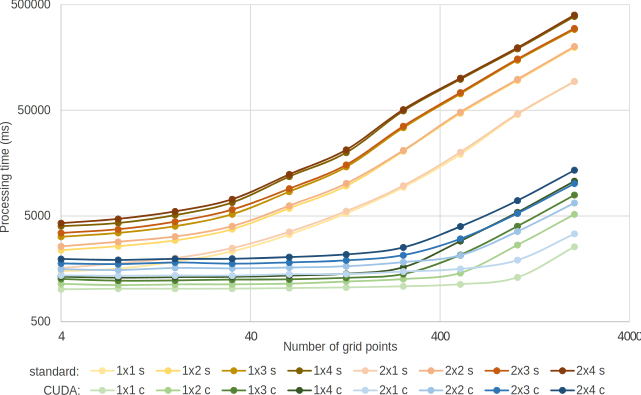
\includegraphics[width=130mm]{figures/cuda-timing.pdf}
	\caption{Computing time for the extraction of analogs over 32 years using the $S_{1}$ criteria for different grid sizes and various structures of AMs. An LxP code represents the structures, with L being the number of levels of analogy and P being the number of predictors per level. Time is given for using (s) standard CPUs and (c) CUDA on GPUs (NVIDIA GeForce RTX 2080). Note the logarithmic axes.}
	\label{cuda}
\end{figure}

The experiment was conducted on the UBELIX cluster of the University of Bern, using the same node for the whole benchmark and processing on a single NVIDIA GeForce RTX 2080 graphics card. The CPU processing -- using the linear algebra library Eigen 3 \cite{Guennebaud2010} -- was done on a single thread. Although AtmoSwing can parallelize the calculation of the analogy criteria on multiple CPU threads, it uses a single thread for this task when optimizing with GAs because it parallelizes the evaluation of the different individuals on multiple threads. With GPUs, it still assesses the individuals on multiple CPU threads, each of them being able to use a different GPU device to calculate the analogy criteria. It is thus parallelizing both on CPUs and GPUs.

The benchmark (Fig. \ref{cuda}) shows that the GPU computations are systematically faster than those on the CPU, and this difference increases with the number of grid points. The GPU computations were 13 times faster on average and up to 38 times faster (5.2~sec instead of 3.3~min) when using 2048 points. Model outputs and reanalyses show an increase in spatial resolution; thus, the impact on the computation time will become increasingly important. When using CPU only, adding a predictor in the first level of analogy has a much higher impact on time than adding a second level of analogy. It is explained by the fact that it needs to process the analogy criteria for the whole archive for each predictor of the first level of analogy, while the second level has only a few candidate situations to assess.



\section{Performance of the Mutation Operators}

As suggested in \citeA{Horton2017a}, five variants of the mutation operator were used in parallel optimizations:

\begin{enumerate}
	\item Chromosome of adaptive search radius \cite{Horton2017a}
	\item Multiscale mutation \cite{Horton2017a}
	\item Non-uniform mutation ($p_{mut}$=0.1, $G_{m,r}$=50, $w$=0.1)
	\item Non-uniform mutation ($p_{mut}$=0.1, $G_{m,r}$=100, $w$=0.1)
	\item Non-uniform mutation ($p_{mut}$=0.2, $G_{m,r}$=100, $w$=0.1)
\end{enumerate}

where $p_{mut}$ is the mutation probability, $G_{m,r}$ is the maximum number of generations (G) during which the magnitude of the research varies, and $w$ is a chosen threshold to maintain a minimum search magnitude when $G>G_{m,r}$.

Figure \ref{fig_mutation_operators_perfs} shows the performance of these five mutation operators for different AM structures and the different catchments considered in Sect. \ref{structures}. Overall, the chromosome of adaptive search radius has a success rate of 76.25\% in calibration and 62.5\% in validation, the multiscale mutation 7.5\%, and 8.75\% respectively, and the non-uniform mutation with its different options: (3) 11.25\% and 10\%, (4) 11.25\% and 21.25\%, and (5) 1.25\% and 2.5\% respectively.

\begin{figure}[hbt]
	\noindent\makebox[\textwidth]{
		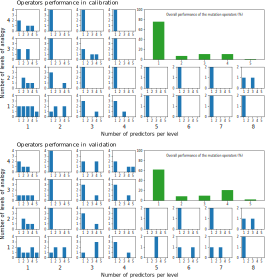
\includegraphics[width=170mm]{figures/gas-configs-ams-structures.pdf}
	}
	\caption{Performance of the five mutation operators (Sect. \ref{gas}) for different AM structures and the different catchments considered in Sect. \ref{structures}. The values represent the number of optimizations for one mutation operator that resulted in the best performing AM. Results are shown for both calibration and validation. When multiple operators obtain the same skill score, they all get a point.}
	\label{fig_mutation_operators_perfs}
\end{figure}

Thus, it is quite clear that the chromosome of adaptive search radius obtains the best results, all the more so with more complex structures, i.e., more predictor variables. Although its success rate decreases slightly in validation, it remains much larger than the other options. The non-uniform mutation shows significant variability of performance depending on its options.

\FloatBarrier

\section{An Attempt to Constrain the Algorithms}

An additional experiment has been attempted by pre-selecting the predictor variables (along with their vertical level and their time) and the analogy criteria and letting the GAs optimize the weights between these variables, along with the spatial domains. To this end, 26 of the most commonly selected ERA5 variables were provided to the optimizer, organized in a single level of analogy. The results are shown in Figure \ref{fig_variables_homogen} and depict high weight values for W at 600 and 700~hPa. Surprisingly, Z700 based on $S_{2}$ also gets relatively high weight values.

\begin{figure}[H]
	\noindent\makebox[\textwidth]{
		\includegraphics[width=180mm]{figures/preselected-variables-era5.pdf}
	}
	\vspace{-0.8cm}
	\caption{Results of the optimization with preselected 26 variables for the different catchments. (top) The colors represent the analogy criteria, and the size of the dots is proportional to the weight given to the predictor within the range [0.01, 0.2]. (bottom) Boxplot of the weight values for the different variables.}
	\label{fig_variables_homogen}
\end{figure}



\FloatBarrier

\section*{Open Research}
Reanalysis datasets can be obtained from the respective providers (see Acknowledgements). Precipitation data can be obtained from MeteoSwiss (for research purpose only). The software used, AtmoSwing \cite<https://atmoswing.org,>{Horton2019}, is open-source and can be used without restrictions.

\acknowledgments
Precipitation time series were provided by MeteoSwiss. The catchment extents were provided by the Hydrological Atlas of Switzerland (hydrologicalatlas.ch). The ERA-Interim reanalysis was obtained from the ECMWF Data Server at http://apps.ecmwf.int/datasets. The Climate Forecast System Reanalysis (CFSR) was obtained from the Computational \& Information Systems Lab (CISL) Research Data Archive (http://rda.ucar.edu/). The CFSR project is carried out by the Environmental Modeling Center (EMC), National Centers for Environmental Prediction (NCEP). ERA5 (Complete ERA5 global atmospheric reanalysis) was obtained from the C3S climate data store (CDS) at https://cds.climate.copernicus.eu. Calculations were performed on UBELIX (http://www.id.unibe.ch/hpc), the HPC cluster at the University of Bern. 



%% ------------------------------------------------------------------------ %%
%% References and Citations

\bibliography{references}


\end{document}

